\section{Закон Стефана-Больцмана, формула смещения Вина. Формула Рэлея-Джинса. Ограниченность классической теории излучения. Элементы квантового подхода. Формула Планка. }


\subsection{Закон Стефана-Больцмана}
\textbf{Закон Стефана-Больцмана} - закон, связывающий поверхностную плотность излучения абсолютно черного тела (тела, которое при любой температуре поглощает все падающее на него излучение) с его температурой.
\begin{equation}
    P = \sigma T^4,
\end{equation}
где P - мощность излучения единицы поверхности абсолютно черного тела, T - температура, \(\sigma\)  - коэффициент пропорциональности, постоянная Стефана-Больцмана.


Эмпирически получен Стефаном, теоретически обоснован Больцманом методами статистической физики. Отметим, что закон говорит только об интегральной мощности излучения, но ничего не говорит о спектре. А вот о спектре скажет закон Рэлея-Джинса.


\subsection{Формула Рэлея-Джинса}
\textbf{Формула Рэлея-Джинса} - спектр (в данном случае закон распределения излучательной способности по частотам испускаемых волн) теплового излучения абсолютно черного тела при фиксированной температуре. При интегрировании этой формулы по всем частотам получается величина, пропорциональная полной мощности излучения. Закон получен Рэлеем и Джинсом теоретически в рамках классической теории. Записывается как:
\begin{equation}
\label{rj}
    B(\omega, T) = kT\frac{\omega^2}{4\pi^2 c^2},
\end{equation}
где \(B\) - яркость излучения в интервале частот от \(\omega\) до \(\omega + d\omega\), \(T\) - температура абсолютно черного тела, \(c\) - скорость света, \(k\) - постоянная Больцмана, \(\omega\) - циклическая частота световой волны, чей вклад в общее излучение мы смотрим.

\subsection{Ограниченность классической теории излучения}
Попробуем, собственно, проинтегрировать формулу Рэлея-Джинса (\ref{rj}) по всем частотам. Интергал, очевидно, расходится:
\begin{equation}
   P \sim \int_{0}^{\infty}  B(\omega, T) d\omega = \int_{0}^{\infty}  kT\frac{\omega^2}{4\pi^2 c^2}  d\omega \to \infty
\end{equation}
Иными словами, с точки зрения классической теории полная мощность теплового излучения единицы объема абсолютно черного тела при любой температуре бесконечно велика. Данный парадокс получил название ультрафиолетовой катастрофы, так как расходимость интеграла вызвана именно видом спектра излучения при больших частотах (см. рис. \ref{comparison})
\begin{figure}
    \centering
    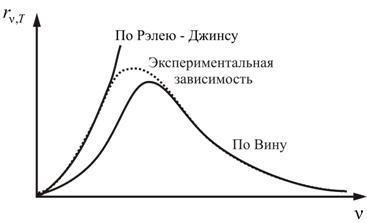
\includegraphics{omparison.jpg}
    \caption{Сравнение законов излучения, о которых пойдет речь в билете}
    \label{comparison}
\end{figure}


\subsection{Элементы квантового подхода, формула Планка и формула смещения Вина}
На помощь по борьбе с парадоксами в классической теории снова приходят кванты. 


\textbf{Формула Планка} - полученный из квантово-статистических соображений закон распределения яркости теплового излучения по частотам при фиксированной температуре абсолютно черного тела. Записывается как:
\begin{equation}
\label{rj}
    B(\omega, T) = \frac{\hbar\omega^3}{4\pi^2 c^2}\frac{1}{\exp(\frac{\hbar\omega}{kT}) - 1},
\end{equation}
Обозначения те же, что и в формуле Рэлея-Джинса. При разложении экспоненты в знаменателе до первого порядка получится формула Рэлея-Джинса. То есть, при малых частотах излучения классическая теория еще работает. Это проиллюстрировано на рис. \ref{comparison} (за не-классический случай отвечает кривая, подписанная 'По Вину', почему так - будет понятно ниже).


\textbf{Закон смещения Вина} устанавливает зависимость частоты волны, на которой поток излучения энергии чёрного тела достигает своего максимума, от температуры чёрного тела. Дифференцируя формулу планка, приравнивая производную к нулю и отбрасывая 'скучные' решения в нуле и на бесконечности, получим запись закона Вина в виде трансцендентного уравнения:
\begin{equation}
    \frac{x\exp^x}{\exp^x - 1} = 5,
\end{equation}
где произведена замена \(x = \frac{\hbar \omega}{kT}\). Численно решив уравнение на \(x\) потом получим параметрическую связь \(\omega_{max}\) и \(T\):
\begin{equation}
    \omega_{max} = \frac{xkT}{\hbar}
\end{equation}
То есть, с ростом температуры линейно растет частота волны, соответствующей максимуму излучения, или, что то же самое, линейно падает длина волны. Это и иллюстрируется графиком \ref{win}.
\begin{figure}
    \centering
    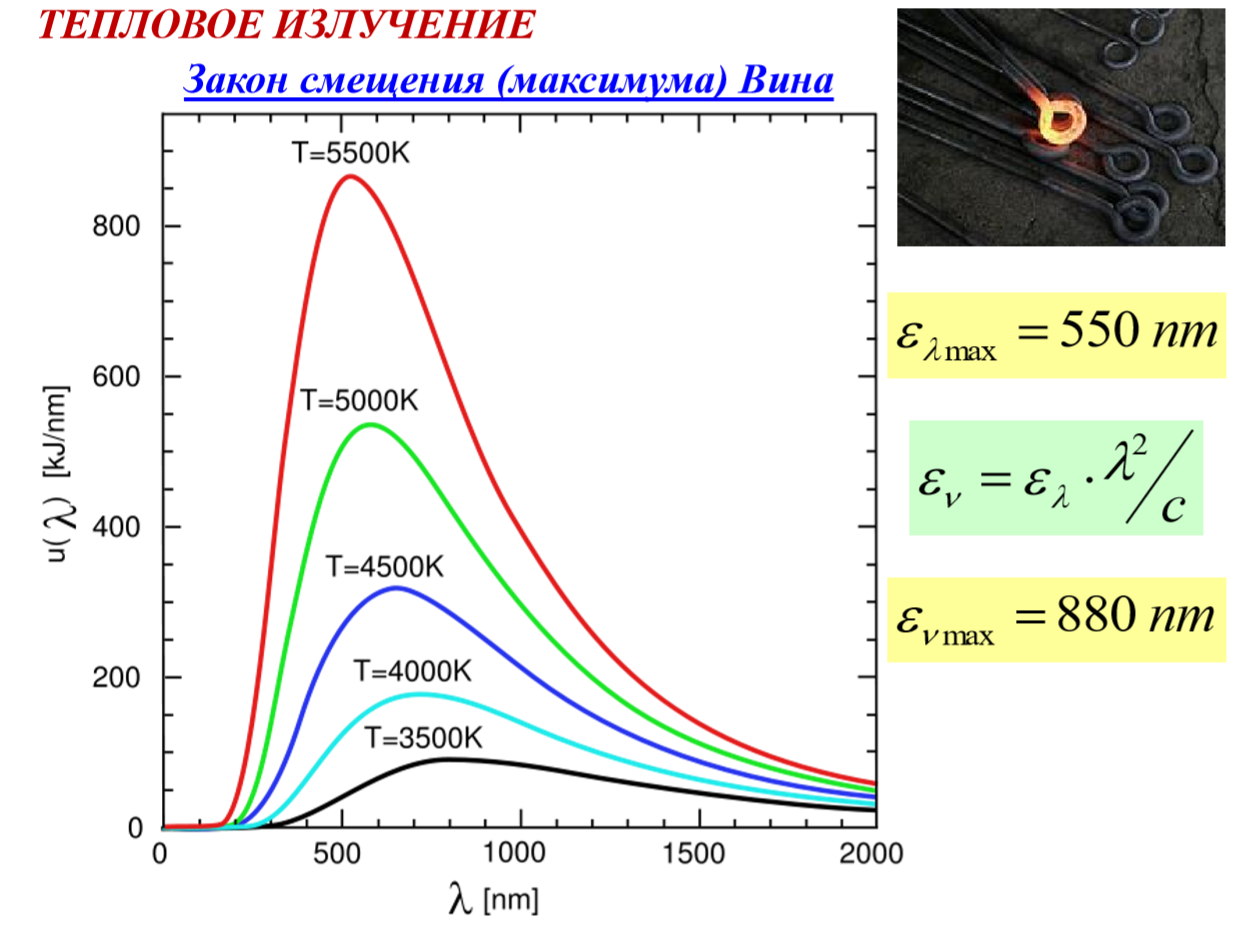
\includegraphics[scale = 0.6]{win.png}
    \caption{Слайд лектора}
    \label{win}
\end{figure}
